\documentclass{article}

\usepackage{fancyhdr}
\usepackage{extramarks}
\usepackage{amsmath}
\usepackage{amsthm}
\usepackage{amsfonts}
\usepackage{tikz}
\usepackage[plain]{algorithm}
\usepackage{algpseudocode}
\usepackage{enumitem}

\usetikzlibrary{automata,positioning}

%
% Basic Document Settings
%

\topmargin=-0.45in
\evensidemargin=0in
\oddsidemargin=0in
\textwidth=6.5in
\textheight=9.0in
\headsep=0.25in

\linespread{1.1}

\pagestyle{fancy}
\lhead{\hmwkAuthorName}
\chead{\hmwkClass\ (\hmwkClassInstructor): \hmwkTitle}
\rhead{\firstxmark}
\lfoot{\lastxmark}
\cfoot{\thepage}

\renewcommand\headrulewidth{0.4pt}
\renewcommand\footrulewidth{0.4pt}

\setlength\parindent{0pt}

%
% Create Problem Sections
%

\newcommand{\enterProblemHeader}[1]{
    \nobreak\extramarks{}{Problem \arabic{#1} continued on next page\ldots}\nobreak{}
    \nobreak\extramarks{Problem \arabic{#1} (continued)}{Problem \arabic{#1} continued on next page\ldots}\nobreak{}
}

\newcommand{\exitProblemHeader}[1]{
    \nobreak\extramarks{Problem \arabic{#1} (continued)}{Problem \arabic{#1} continued on next page\ldots}\nobreak{}
    \stepcounter{#1}
    \nobreak\extramarks{Problem \arabic{#1}}{}\nobreak{}
}

\setcounter{secnumdepth}{0}
\newcounter{partCounter}
\newcounter{homeworkProblemCounter}
\setcounter{homeworkProblemCounter}{1}
\nobreak\extramarks{Problem \arabic{homeworkProblemCounter}}{}\nobreak{}

%
% Homework Problem Environment
%
% This environment takes an optional argument. When given, it will adjust the
% problem counter. This is useful for when the problems given for your
% assignment aren't sequential. See the last 3 problems of this template for an
% example.
%
\newenvironment{homeworkProblem}[1][-1]{
    \ifnum#1>0
        \setcounter{homeworkProblemCounter}{#1}
    \fi
    \section{Problem \arabic{homeworkProblemCounter}}
    \setcounter{partCounter}{1}
    \enterProblemHeader{homeworkProblemCounter}
}{
    \exitProblemHeader{homeworkProblemCounter}
}

%
% Homework Details
%   - Title
%   - Due date
%   - Class
%   - Section/Time
%   - Instructor
%   - Author
%

\newcommand{\hmwkTitle}{Homework\ \#3}
\newcommand{\hmwkDueDate}{October 6, 2017}
\newcommand{\hmwkClass}{STAT 310}
\newcommand{\hmwkClassInstructor}{Guerra}
\newcommand{\hmwkAuthorName}{\textbf{Joel Abraham}}

%
% Title Page
%

\title{
    \vspace{2in}
    \textmd{\textbf{\hmwkClass:\ \hmwkTitle}}\\
    \normalsize\vspace{0.1in}\small{Due\ on\ \hmwkDueDate\ at 5:00 PM}\\
    \vspace{0.1in}\large{\textit{\hmwkClassInstructor}}
    \vspace{3in}
}

\author{\hmwkAuthorName}
\date{}

\renewcommand{\part}[1]{\textbf{\large Part \Alph{partCounter}}\stepcounter{partCounter}\\}

%
% Various Helper Commands
%

\newcommand{\liminfty}{\lim\limits_{y\to\infty}}

\newcommand{\limninf}{\lim\limits_{y\to-\infty}}

% Useful for algorithms
\newcommand{\alg}[1]{\textsc{\bfseries \footnotesize #1}}

% For derivatives
\newcommand{\deriv}[1]{\frac{\mathrm{d}}{\mathrm{d}x} (#1)}

% For partial derivatives
\newcommand{\pderiv}[2]{\frac{\partial}{\partial #1} (#2)}

% Integral dx
\newcommand{\dx}{\mathrm{d}x}

% Alias for the Solution section header
\newcommand{\solution}{\textbf{\large Solution}}

% Probability commands: Expectation, Variance, Covariance, Bias
\newcommand{\E}{\mathbb{E}}
\newcommand{\Var}{\mathrm{Var}}
\newcommand{\Cov}{\mathrm{Cov}}
\newcommand{\Bias}{\mathrm{Bias}}

\begin{document}

\maketitle
\pagebreak

\begin{homeworkProblem}
    RT 2.5.5. The cumulative distribution function $F(x)$ of a random variable $X$ is given by 
    \[ F(x) = 
    \begin{cases} 
        0, & -\infty < x < -1 \\
        0.2, & -1 \leq x < 3 \\
        0.8, & 3 \leq x < 9 \\
        1, & x \geq 9
    \end{cases}
    \]
    Write down the values of the random variable $X$ and the corresponding probabilities $p(x)$. Also find $\E[X]$ and SD(X). \\

    \textbf{Solution}
    \[ p(x) = 
    \begin{cases} 
        0.2, & x = -1 \\
        0.6, & x = 3 \\
        0.2, & x = 9 \\
        0, & otherwise
    \end{cases}
    \]. Then, $\E[X] = (-1)(0.2) + (3)(0.6) + (9)(0.2) = -0.2 + 1.8 + 1.8 = 3.4.$ $\Var(X) = \sigma^2 = \E[X^2] - (\E[X])^2 = (1)(0.2) + (9)(0.6) + (81)(0.2) + 3.4^2 = 0.2 + 5.4 + 16.2 - 11.56 = 10.24 \implies SD(X) = \sqrt{10.24} = 3.2$.
    
    
    

\end{homeworkProblem}



\begin{homeworkProblem}
    Rose is planning a dinner party for seven guests. All her invited friends will be assistant professors, all of whom are working 16 hours a day to get tenure. Being so busy with their careers, each professor will accept the invitation according to the flip of a fair coin: heads accept, tails don’t accept the invitation. Rose also knows that each professor that accepts the invitation will actually attend with chance 80\%. Rose decides to invite 12 professors. The professors have almost no social life so they will make decisions independently of each other. What is the probability that Rose will end up with more professors than she can accommodate?
    \\
    
    \textbf{Solution} \\
    
    The probability of a professor attending is P(A) = (0.5)(0.8) = 0.4, where A is the event that a professor attends. Thus, we want to find the probability of 8 or more professors attending. Since this follows a binomial distribution, we have (where M is the event that Rose ends up with  more professors than she can accommodate) \[P(M) = \sum_{k=8}^{12} {12 \choose k}(0.4)^k(0.6)^{12-k} \implies\]\[P(M) = {12 \choose 8}(0.4)^8(0.6)^4 + {12 \choose 9}(0.4)^9(0.6)^3 + {12 \choose 10}(0.4)^10(0.6)^2 + {12 \choose 11}(0.4)^11(0.6)^1 + {12 \choose 12}(0.4)^12 \implies\]
    \[P(M) = 0.0573\].

\end{homeworkProblem}

\begin{homeworkProblem}
    ACT and SAT college entrance exams are taken by thousands of students each year. The mathematics scores on each exam are normally distributed. In recent years, the SAT math scores have had a mean of 480 and SD of 100, while the ACT mean and SD are 18 and 6, respectively. For purposes of this exercise, assume SAT scores range from 400 to 800 and ACT scores range from 1 to 36.
    \begin{enumerate}[label=(\alph*)]
        \item A certain engineering program has a minimum SAT math score of 600 for admission. What percentage of students are eligible for the program?
        
        \item What is a comparable ACT standard for admission to the engineering program?
        
        \item The engineering program accepts 30 students per year. How many of these 30 students are expected to have an SAT math score of 750 or higher?
    \end{enumerate}
    
    \textbf{Solution}
    \begin{enumerate}[label=(\alph*)]
        \item The probability density function for the normally distributed SAT math scores is given by 
        \[f(x) = \frac{1}{\sqrt{2\pi}\sigma}e^{-\frac{1}{2}(\frac{x-\mu}{\sigma})^2}\]. Thus, for $\mu = 480$ and $\sigma = 100$, we have
        \[f(x) = \frac{1}{100\sqrt{2\pi}}e^{-\frac{1}{2}(\frac{x-480}{100})^2}\]. We now consider 
        \[F(x) = \int_{-\infty}^{x}f(x)dx = \int_{-\infty}^{x}\frac{1}{100\sqrt{2\pi}}e^{-\frac{1}{2}(\frac{x-480}{100})^2}dx\]
        \[P(X \geq 600) = 1 - P(X < 600) = 1 - F(600) = \int_{600}^{\infty}\frac{1}{100\sqrt{2\pi}}e^{-\frac{1}{2}(\frac{x-480}{100})^2}dx = 0.115.\]
        We compute this using the R command: pnorm(600, mean=480, sd=100, lower.tail = FALSE) = 0.115.
        
        \item A comparable ACT score is given by: qnorm(0.1150697, mean=18, sd=6, lower.tail = FALSE) = $25.2 \approx 25$
        
        \item Let A represent the event that a student has an SAT math score greater than or equal to 750 and let B represent the event that a student has an SAT math score greater than or equal to 600 (is accepted into the engineering program). Now, $P(A)$ = pnorm(750, mean=480, sd=100, lower.tail = FALSE) = $0.00347$ and $P(B) = 0.115$. Then, \[P(A|B) = \frac{P(A \cap B)}{P(B)} = \frac{0.00347}{0.115} = 0.0301.\] Thus, we would expect $0.0301*30 = 0.904 \approx 1$ student in the engineering program to score 750 or higher.
        
        
    \end{enumerate}
\end{homeworkProblem}

\begin{homeworkProblem}
    A jury of 12 persons is to be selected from a pool of 25 persons called to jury duty. The pool of 25 persons includes 12 retired persons, 6 employed persons, 2 unemployed and 5 students. Assume that each person is equally likely to be selected.
    \begin{enumerate}[label=(\alph*)]
        \item What is the probability that two students will be selected?
        
        \item What is the probability that at least half the jury will be comprised of retired persons?
        
        \item What is the probability that the jury will contain exactly twice as many retired persons as employed persons?
    \end{enumerate}
    
    \textbf{Solution} \\
    \begin{enumerate}[label=(\alph*)]
        \item Let T represent the event that exactly two students are selected. Then, P(T) is the number of ways we can choose a jury with two students divided by the number of total juries. This is given by \[P(T) = \frac{\binom{5}{2}\binom{20}{10}}{\binom{25}{12}} = 0.355\]
        
        \item The probability that at least half the jury is composed of retired persons (which we label event R) is the probability that the jury has 6 - 12 retired persons. Then, we have 
        \[P(R) = \sum_{k=6}^{12} \frac{\binom{12}{k}\binom{13}{12-k}}{\binom{25}{12}} = \frac{\binom{12}{6}\binom{13}{6}}{\binom{25}{12}} + \frac{\binom{12}{7}\binom{13}{5}}{\binom{25}{12}} + \frac{\binom{12}{8}\binom{13}{4}}{\binom{25}{12}} + ... + \frac{1}{\binom{25}{12}} = 0.582\]
        
        \item Let E be the event that the jury contains exactly twice as many retired people as employed people. Then, the jury can have 2, 3, or 4 employed people, and 2, 4, 6, or 8 retired people, respectively. Thus, 
        \[P(E) = \sum_{k=2}^{4} \frac{\binom{6}{k}\binom{12}{2k}\binom{7}{12 - 3k}}{\binom{25}{12}} =  \frac{\binom{6}{2}\binom{12}{4}\binom{7}{6}}{\binom{25}{12}} + \frac{\binom{6}{3}\binom{12}{6}\binom{7}{3}}{\binom{25}{12}} + \frac{\binom{6}{4}\binom{12}{8}}{\binom{25}{12}} = 0.136\]
    \end{enumerate}
\end{homeworkProblem}

\begin{homeworkProblem}
    Let Y $\sim$ Exp($\beta$). Show that Y has a memoryless property. Thus, if $s \geq 0$ and $t \geq 0$, then
    \[P(Y > s+t| Y > s) = P(Y > t)\]
    
    \textbf{Solution} \\
    Since Y $\sim$ Exp($\beta$), we have $f(x) = \frac{1}{\beta}\mathrm{e}^{\frac{-x}{\beta}}$. And, $P(Y > s+t| Y > s) = \frac{P(Y > s+t)}{P(Y > s)}$. First, note that:
    \[P(Y > a) = \int_{a}^{\infty}f(x)dx = \int_{a}^{\infty}\frac{1}{\beta}\mathrm{e}^{\frac{-x}{\beta}}dx = \left[-\mathrm{e}^{\frac{-x}{\beta}}\right]_{a}^{\infty} = -\mathrm{e}^{\frac{-\infty}{\beta}} + \mathrm{e}^{\frac{-a}{\beta}} = \mathrm{e}^{\frac{-a}{\beta}}.\] Thus, we have 
    \[\frac{P(Y > s+t)}{P(Y > s)} = \frac{\mathrm{e}^{\frac{-s-t}{\beta}}}{\mathrm{e}^{\frac{-s}{\beta}}} = \mathrm{e}^{\frac{-s-t}{\beta} + \frac{s}{\beta}} = \mathrm{e}^{\frac{s-s-t}{\beta}} = \mathrm{e}^{\frac{-t}{\beta}} = P(Y > t).\]
\end{homeworkProblem}

\begin{homeworkProblem}
    The number of arrivals $N$ at a supermarket checkout counter in the time interval from 0 to t follows a Poisson distribution with mean $\lambda$t. Let T denote the length of time until the first arrival. Find the probability density function of T. Hint: Consider $P(T > t_0)$. \\
    
    \textbf{Solution} \\
    
    Since we know that arrivals follow a Poisson distribution, we have \[P(N = n) = \frac{\mathrm{e}^{-\lambda t}(\lambda t)^n}{n!}.\] Now, we seek to find \[F(t) = P(T < t) = 1 - P(T > t).\] Since T is the length of time until the first arrival, $P(T > t)$ is the probability that the first arrival occurs after some time $t$, which is equivalent to the probability that no arrivals occur between time $0$ and $t$. Thus, \[P(T > t) = P(N = 0) = \frac{\mathrm{e}^{-\lambda t}(\lambda t)^0}{0!} = \mathrm{e}^{-\lambda t} \implies F(t) = P(T < t) = 1 - e^{-\lambda t}.\] Since the probability density function is the derivative of the cumulative distribution function, we have \[f(t) = \frac{\mathrm{d}}{\mathrm{d}t}F(t) = \lambda\mathrm{e}^{-\lambda t}.\]
    
\end{homeworkProblem}

\begin{homeworkProblem}
    Let Y by a continuous random variable with pdf, $f(y$), and cdf, $F(y)$. We are often interested in conditional probabilities of the form $P(Y \leq y|Y \geq c)$. For example, the probability that cell phone battery will last less than 3 years, given that it is now 1 year old.
    
    \begin{enumerate}[label=(\alph*)]
        \item Show that for $y \geq c$,
        \[F_c(y) = P(Y \leq y|Y \geq c)= \frac{F(y)-F(c)}{1 - F(c)}\]
        
        \item Show that the above function satisfies all the properties of a distribution function. (a) $F_c(y)$ approaches 0 as $y \implies -\infty$. (b) $F_c(y)$ approaches 1 as $y \implies \infty$. (c) $F_c(y)$ is non-decreasing; for $y_1 < y_2$, then $F_c(y_1) \leq F_c(y_2)$.
        
        \item Since $F_c(y)$ is a distribution function of a continuous r.v., then it has a pdf. Show that the pdf is
        
        \[f_c(y)= \frac{f(y)}{1 - F(c)}, y \geq c.\]
        
        
        \item Suppose you are waiting for a call back from a job interview. Assume the waiting time for the
        call back, Y, follows an exponential distribution with mean 24 hours.
        
        \begin{enumerate}[label=(\roman*)]
            \item What is chance that you will get the call within 24 hours?
            
            \item What is the expected value of Y?
            
            \item Given that 8 hours have already passed, what is the chance that you will get the call within
            24 hours?
            
            \item Given that 8 hours have already passed, what is the expected value of Y ?
        \end{enumerate}
    \end{enumerate}
    \textbf{Solution}
    
    \begin{enumerate}[label=(\alph*)]
        \item For $y \geq c$,
        \[P(Y \leq y|Y \geq c) = \frac{P(c \leq Y \leq y)}{P(Y \geq c)}.\] $P(Y \geq c) = 1 - P(Y < c) = 1 - F(c)$, and \[P(Y \leq y|Y \geq c) = \int_{c}^{y}f(x)dx = \int_{c}^{-\infty}f(x)dx + \int_{-\infty}^{y}f(x)dx = F(y) - F(c).\] Thus, we have \[F_c(y) = P(Y \leq y|Y \geq c) = \frac{F(y) - F(c)}{1 - F(c)}\]
        
        \item Since $F$ is a distribution function, we know $\lim\limits_{x\to\infty} F(x) = 1$ and $\lim\limits_{x\to-\infty} F(x) = 0$, thus
        \[\liminfty F_c(y) = \liminfty \frac{F(y) - F(c)}{1 - F(c)} = \frac{\liminfty F(y) - F(c)}{1 - F(c)} = \frac{1 - F(c)}{1 - F(c)} = 1.\] For the case when y approaches $-\infty$, we have $y < c$, thus $F_c(y) = 0$ since $P(Y \leq y|Y \geq c) = 0$ because when $y < c$, we have $P(Y \leq y \cap Y \geq c) = P(Y < c \cap Y \geq c) = P(\emptyset) = 0$. Now, we show that $F_c(y)$ is nondecreasing since $F(x)$ is nondecreasing. For $y_1 < y_2$, we have
        \[F(y_1) \leq F(y_2) \implies F(y_1) - F(c) \leq F(y_2) - F(c) \implies \frac{F(y_1) - F(c)}{1 - F(c)} \leq \frac{F(y_2) - F(c)}{1 - F(c)} \implies F_c(y_1) \leq F_c(y_2).\]
        
        \item The probability distribution function is the derivative of the cumulative distribution, so we first observe that
        \[F_c(y) = \frac{F(y)}{1 - F(c)} - \frac{F(c)}{1 - F(c)},\] thus since $(1 - F(c))^{-1}$ is a constant,
        \[f_c(y) = \frac{\mathrm{d}}{\mathrm{d}y}F_c(y) = \frac{\mathrm{d}}{\mathrm{d}y}(\frac{F(y)}{1 - F(c)}) = \frac{f(y)}{1 - F(c)}, y \geq c\]
        
        \item $Y \sim$ Exp($\beta$), where $\beta = 24$
            \begin{enumerate}[label=(\roman*)]
                \item The chance of a callback within 24 hours is equal to 
                \[F(24) = \int_{0}^{24}\frac{1}{24}\mathrm{e}^{\frac{-x}{24}}dx = \left[1 - \mathrm{e}^{\frac{-x}{24}}\right]_0^{24} = 1 - \frac{1}{\mathrm{e}}\]
                
                \item The expected value is equivalent to the mean, thus $\E[Y] = \beta = 24$
                
                \item We use the definition of $F_8(y)$ as follows. We must first calculate $F(8) = 1- \mathrm{e}^{-\frac{1}{3}}$, thus \[F_8(24) = \frac{F(24) - F(8)}{1 - F(8)} = \frac{1 - \mathrm{e}^{-1} - (1 - \mathrm{e}^{-\frac{1}{3})} - }{1 - (1 - \mathrm{e}^{-\frac{1}{3}})} =  \frac{\mathrm{e}^{-\frac{1}{3}} - \mathrm{e}^{-1}}{\mathrm{e}^{-\frac{1}{3}}} = 1 - \mathrm{e}^{(-1 + \frac{1}{3})} = 1 - \mathrm{e}^{-\frac{2}{3}}\]
                
                \item Given that 8 hours have passed, we define \[F_8(y) = 1 - \mathrm{e}^{(\frac{8-y}{24})}.\] Thus, by linearity of expectation and part (b), we have
                \[\E[Y] = \int_{0}^{\infty} yf_8(y)dy = \int_{0}^{\infty} \frac{yf(y)}{1 - F(8)}dy = \frac{1}{1 - F(8)}\int_{0}^{\infty} f(y)dy  = \mathrm{e}^{-\frac{1}{3}}\int_{0}^{\infty} yf(y)dy = 24\mathrm{e}^{-\frac{1}{3}} = 17.197\]
            \end{enumerate}
    \end{enumerate}
\end{homeworkProblem}

\begin{homeworkProblem}
    Problem 3.4. Severe snow storm is defined as a storm whose snowfall exceeds 10 inches. Let X be the amount of snowfall in a severe snow storm. The cumulative distribution function (CDF) of X in a given town is:
    \[F_x(x) = \begin{cases}
                    1 - (\frac{10}{x})^4 &  x \geq 10 \\
                    0 & x < 10
                \end{cases}\]
    \begin{enumerate}[label=(\alph*)]
        \item Determine the median of X.
        \item What is the expected amount of snowfall in the town in a severe snow storm?
        \item Suppose a disastrous snow storm is defined as a storm with over 15 inches of snowfall. What percentage of the severe snow storms are disastrous?
        \item Suppose the probability that the town will experience 0, 1, and 2 severe snow storms in a year is 0.5, 0.4, and 0.1, respectively. Determine the probability that the town will not experience a disastrous snow storm in a given year. Assume the amounts of snowfall between storms are statistically independent. 
    \end{enumerate}
    \textbf{Solution}
    \begin{enumerate}[label=(\alph*)]
        \item The median is the point at which $F_x(x) = 0.5$, thus 
        \[1 - (\frac{10}{x})^4 = 0.5 \implies (\frac{10}{x})^4 = 0.5 \implies \frac{10}{x} = (0.5)^{0.25} \implies x = \frac{10}{(0.5)^{0.25}} \implies x = 11.892.\]
        
        \item The density function is given by
        \[f(x) = \deriv F_x(x) = \deriv 1 - \frac{10^4}{x^{4}} = 4(\frac{10^4}{x^5}).\] Thus, we calculate expected value via:
        \[\E[X] = \int_{10}^{\infty} xf(x)dx = 4*10^4 \int_{10}^{\infty} \frac{1}{x^4}dx = -\frac{4}{3}*10^4\left[\frac{1}{x^3}\right]_{10}^{\infty} = \frac{4}{3}*10^4\frac{1}{10^3} = 13.333\]
        
        \item We find the probability that a severe snow storm is disastrous by
        \[P(X > 15) = 1 - P(X <= 15) = 1 - F_x(15) = 1 - (1 - (\frac{2}{3})^4) = (\frac{2}{3})^4 = 0.1975\]
        
        \item The probability that a severe snow storm is not disastrous is $P(X \leq 15) = 1 - 0.1975 = 0.802$. Thus, the probability of no disastrous storms is given by $P(D = 0) = 0.5*(1) + 0.4*(0.802) + 0.1*(0.802)^2 = 0.885$.
    \end{enumerate}
\end{homeworkProblem}

\begin{homeworkProblem}
    Problem 3.12. The total load, X (in tons), on the roof of a building has the following PDF:
    \[f_x(x) = \begin{cases}
                    \frac{24}{x^3} &  3 \leq x \leq 6 \\
                    0 & otherwise
                \end{cases}\]
    \begin{enumerate}[label=(\alph*)]
        \item Determine and plot the CDF of X, i.e., $F_x(x)$.
        \item What is the expected total load?
        \item Determine the coefficient of variation of the total load.
        \item Suppose the roof can carry only 5.5 tons before collapse. What is the probability that the roof will collapse?
    \end{enumerate}
    
    \textbf{Solution}
    \begin{enumerate}[label=(\alph*)]
        \item \[F_x(x) = \int_{-\infty}^{x}f_x(x)dx = \int_{3}^{x}f_x(x)dx = 24\int_{3}^{x}\frac{1}{x^3}dx = -12\left[\frac{1}{x^2}\right]_3^x = -\frac{12}{x^2} + \frac{4}{3}.\]
        Thus, 
        \[F_x(x) = \begin{cases}
                    0 & x < 3 \\
                    -\frac{12}{x^2} + \frac{4}{3} &  3 \leq x \leq 6 \\
                    1 & x > 6
                \end{cases}\]
        
        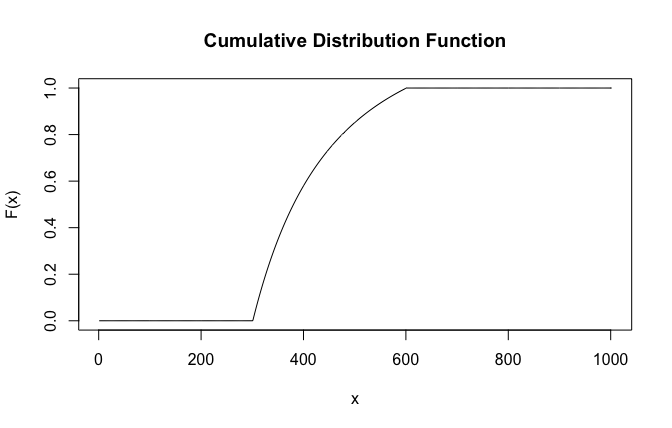
\includegraphics[scale=.6]{cdf.png}
        
        \item The expected value of the total load is given by 
        \[\E[X] = \int_{3}^{6}xf_x(x)dx = 24\int_{3}^{6}\frac{1}{x^2}dx = 24\left[-\frac{1}{x}\right]_3^6 = 24[-\frac{1}{6} +\frac{1}{3}] = 4\]
        
        \item The variance is given by 
        \[\Var[X] = \E[X^2] - \E[X]^2 = -\E[X]^2 + \int_{3}^{6}x^2f_x(x)dx = 24\int_{3}^{6}\frac{1}{x}dx - 16 = 24\left[\ln{x}\right]_3^6 - 16=  24\ln{2} - 16\] Thus since $\E[X] = 4$, we can calculate coefficient of variation as
        \[CV = \frac{\sigma}{\mu} = \frac{\sqrt{\Var[X]}}{{\E[X]}} = \frac{\sqrt{24\ln{2} - 16}}{{4}} = 0.199\]
        
        \item The probability that the roof will collapse is the probability that the load is greater than 5.5 tons, thus 
        \[P(X > 5.5) = 1 - P(X \leq 5.5) = 1 - F_x(5.5) = 1 + \frac{12}{5.5^2} - \frac{4}{3} = 0.0633\]
    \end{enumerate}
\end{homeworkProblem}

\end{document}
